
We wanted to keep the preprocessing part of our algorithm simple as we found the other stages of the human face authentication pipeline more interesting. In hindsight though we recognize that this phase becomes the foundation determining the amount of work as well as the performance of the other phases. Therefore we should perhaps have put more effort into implementing an algorithm that works better for various lightning conditions and that also normalizes the colors better. An improved version could for example have led to that the proposed algorithm would have been able to correctly detect the face seen in Figure \ref{fig:fail2}. 

\begin{figure}[H]
\centering

\begin{subfigure}{.25\textwidth}
  \centering
  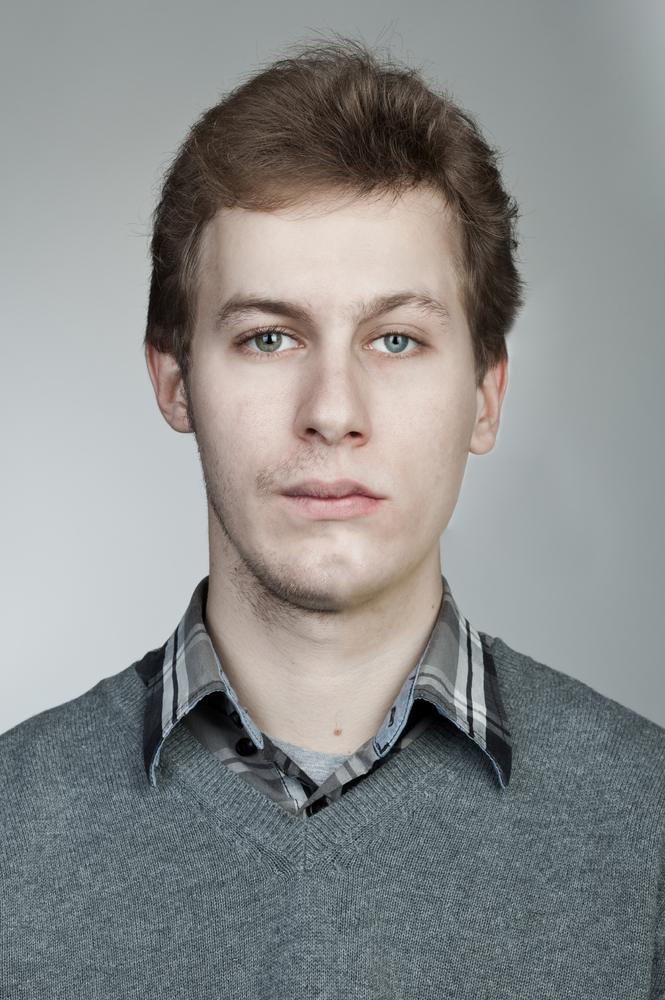
\includegraphics[width=0.53\textwidth]{img/fd3/fail2_input.jpg}
  \caption{}
\end{subfigure}%
\begin{subfigure}{.25\textwidth}
  \centering
  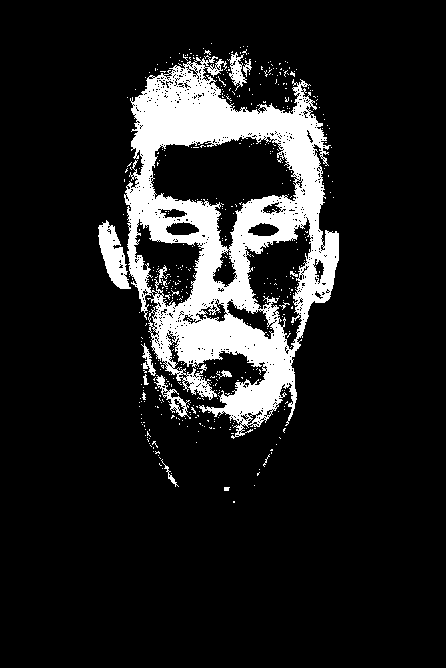
\includegraphics[width=0.53\textwidth]{img/fd3/fail2_estimatedSkinMak.png}
  \caption{}
\end{subfigure}%
\begin{subfigure}{.25\textwidth}
  \centering
  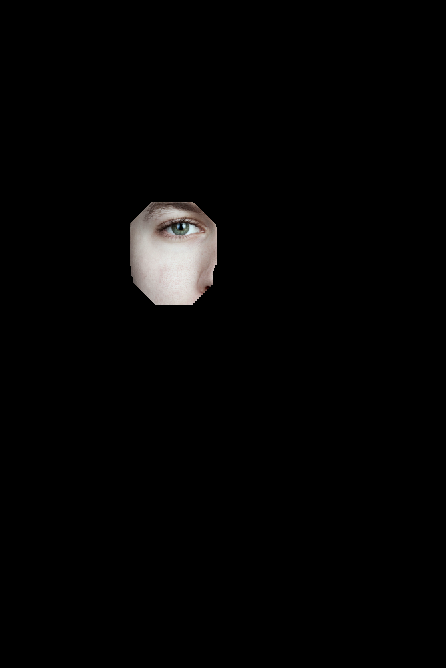
\includegraphics[width=0.53\textwidth]{img/fd3/fail2_faceImage.png}
  \caption{}
\end{subfigure}%
\begin{subfigure}{.25\textwidth}
  \centering
  
\includegraphics[width=0.23\textwidth]{img/fd3/fail2_output.png}
  \caption{}
\end{subfigure}%

\caption{A case where the proposed algorithm fails to detect the correct face due to a too sparse estimated skin mask. (a) show the input face, (b) the estimated skin mask, (c) the resulting invalid face mask and (d) the output.}
\label{fig:fail2}
\end{figure}

For face detection we decided to go by the article in \cite{fdInColorImages} that is based on the extraction of eyes and mouth through the use of the relations between colors in faces. However we also looked into algorithms that require training and uses features, like the \textit{Viola Jones} \cite{viola} algorithm.

The aim of the segmentation steps taken during the face detection phase were to reduce the search space for the Circular Hough Transform when looking for the eyes. We do though recognize that this process might be overly complicated as the single purpose for it is to make it easier to locate the eyes. Although we tried to extract the eyes directly from the original eye map (Figure 7\textit{c}) in various ways, for example by thresholding while taking the mean value and the variance into consideration, we did not found one that was satisfying. We do however believe that a better preprocessing stage could have mitigated this problem.

Another method we looked into were to utilize the ability of Eigenfaces and its face space in order to recognize whether a blob found, in for example the mask of Figure 4\textit{f}, were an actual face or not. However we left the implementation this method for a future study.

Furthermore do we believe that dynamic thresholds and kernel widths would have made our implementation more robust. Especially in regard to faces and images of few pixels, like those in the given database \textit{db0}. In order to make our implementation less sensitive and more tolerant we have for example been working with circular disks as kernel elements for dilation and erosion and thresholds with large margins. More over do we believe that the face detection part of the algorithm could be improved by utilizing the facial expression methods explored in \cite{facialExpressions}. This as we have found out through experimentation that the mouth plays a large role during the recognition phase. For example when we run tests only including the eyes and nose we received a larger recognition rate.


